\documentclass{beamer}
\usepackage{latexsym}
\usepackage{natbib}
\usepackage{graphicx}
\usepackage{subfigure}
\usepackage{listings}
\usepackage{algorithm}
\usepackage{algpseudocode}
\usepackage{amsmath}
\usepackage{amssymb} 
\usepackage{amsthm}

\newcommand{\R}{\mathbb{R}}
\newcommand{\E}{\mathrm{E}}
\newcommand{\Cov}{\mathrm{Cov}}
\newcommand{\Var}{\mathrm{Var}}


\usetheme{Warsaw}

\title{MCMT Project\\Mixing Time in Reinforcement Learning}
\author{Shun Zhang}

\defbeamertemplate*{footline}{shadow theme}
{%
  \leavevmode%
  \hbox{\begin{beamercolorbox}[wd=.5\paperwidth,ht=2.5ex,dp=1.125ex,leftskip=.3cm plus1fil,rightskip=.3cm]{author in head/foot}%
    \usebeamerfont{author in head/foot}\insertframenumber\,/\,\inserttotalframenumber\hfill\insertshortauthor
  \end{beamercolorbox}%
  \begin{beamercolorbox}[wd=.5\paperwidth,ht=2.5ex,dp=1.125ex,leftskip=.3cm,rightskip=.3cm plus1fil]{title in head/foot}%
    \usebeamerfont{title in head/foot}
  \end{beamercolorbox}}%
}

\begin{document}

\begin{frame}
\titlepage
\end{frame}

\begin{frame}
\frametitle{What is Reinforcement Learning}
\begin{itemize}
\item Learning with feedback, or sequential decision making.
\item Defined on {\em Markov Decision Process},
\item which is an extension to Markov chain.
\end{itemize}
\end{frame}

\begin{frame}
\frametitle{Definitions}
\begin{definition}
Markov Chain is a two-element tuple $(\Omega, P)$, where
\begin{itemize}
\item $\Omega$ is the state space.
\item $P$ is the transition probability. $P: \Omega \times \Omega \rightarrow
\R$.
\end{itemize}
\end{definition}

\begin{definition}
Markov Decision Process is a four-element tuple $(\Omega, A, P, R)$, where
\begin{itemize}
\item $\Omega$ is the state space.
\item $A$ is an action set.
\item $P$ is the transition probability. $P: \Omega \times A \times \Omega
\rightarrow \R$.
\item $R$ is the reward upon reaching a state. $R: \Omega \rightarrow \R$.
\cite{rl}
\end{itemize}
\end{definition}
\end{frame}

\begin{frame}
\frametitle{Definitions}
\begin{definition}
A policy in a MDP is a mapping $\pi: \Omega \rightarrow A$.
\end{definition}

\begin{definition}
The utility of a state $s$ following policy $\pi$ is: $U(s) = \E (R(s) + \gamma
R(s_1) + \gamma^2 R(s_2) + \cdots)$, where $\gamma \in (0, 1]$, is a discounting
factor.
\end{definition}
\end{frame}

\begin{frame}
\frametitle{Objective}
\begin{itemize}
\item The goal of the agent is to maximize the accumulated rewards it gets.
\item The agent should take the action that leads to the maximum expected
utilities, that is ${\mathrm{argmax}}_a \sum_{s'} P(s, a, s') (R(s') + \gamma
U(s'))$.
\item Explore or Exploit Dilemma ($\epsilon$-greedy, Upper bound confidence interval).
\end{itemize}
\end{frame}

\begin{frame}
\frametitle{Learning algorithms: Value Iteration}
\begin{theorem}
The utility of the optimal policy satisfies $U(s) = \max_a \sum_{s'} P(s, a, s')
(R(s') + \gamma U(s'))$ for all $s$.
\end{theorem}

To update, we can use the following rule. This is a bootstrapping way to solve
the nonlinear equations above.

\begin{equation}\label{eq:vl}
U(s) \leftarrow \max_a \sum_{s'} P(s, a, s') (R(s') + \gamma U(s'))
\end{equation} 
\end{frame}

\begin{frame}
\frametitle{Learning algorithms: Q-learning}
\begin{definition}
$Q(s, a) = \sum_{s'} P(s, a, s') (R(s') + \gamma U(s'))$.
\end{definition}
Note that by definition, $U(s) = \max_a Q(s, a)$. The $Q$ function can be
computed by the following update rule.

\begin{equation}\label{eq:td}
Q(s, a) \leftarrow (1 - \alpha) Q(s, a) + \alpha (R(s') + \gamma \max_{a'} Q(s',
a'))
\end{equation} 
where $\alpha \in (0, 1)$. 

\begin{theorem}
Following the update rule Equation~\ref{eq:td}, $Q$ eventually converges to $Q^*$.
\end{theorem}
\end{frame}

\begin{frame}
\frametitle{Experiments}
One measure of the learning performance is to compare the current utility with
that of the optimal solution, that is $\sum_s ||U(s) - U^*(s)||$ or $\sum_{s,a}
||Q(s, a) - Q^*(s, a)||$ for $s \in \Omega$.
\end{frame}

\begin{frame}
\begin{figure}[h!]
\frametitle{Experiments}
\includegraphics[width=0.7\textwidth]{exp0.pdf}
\caption{Convergence rates of different domains, with sizes of 3x3, 4x4, 5x5.}
\label{fig:exp}
\end{figure}
\end{frame}

\begin{frame}
\begin{figure}[h!]
\frametitle{Experiments}
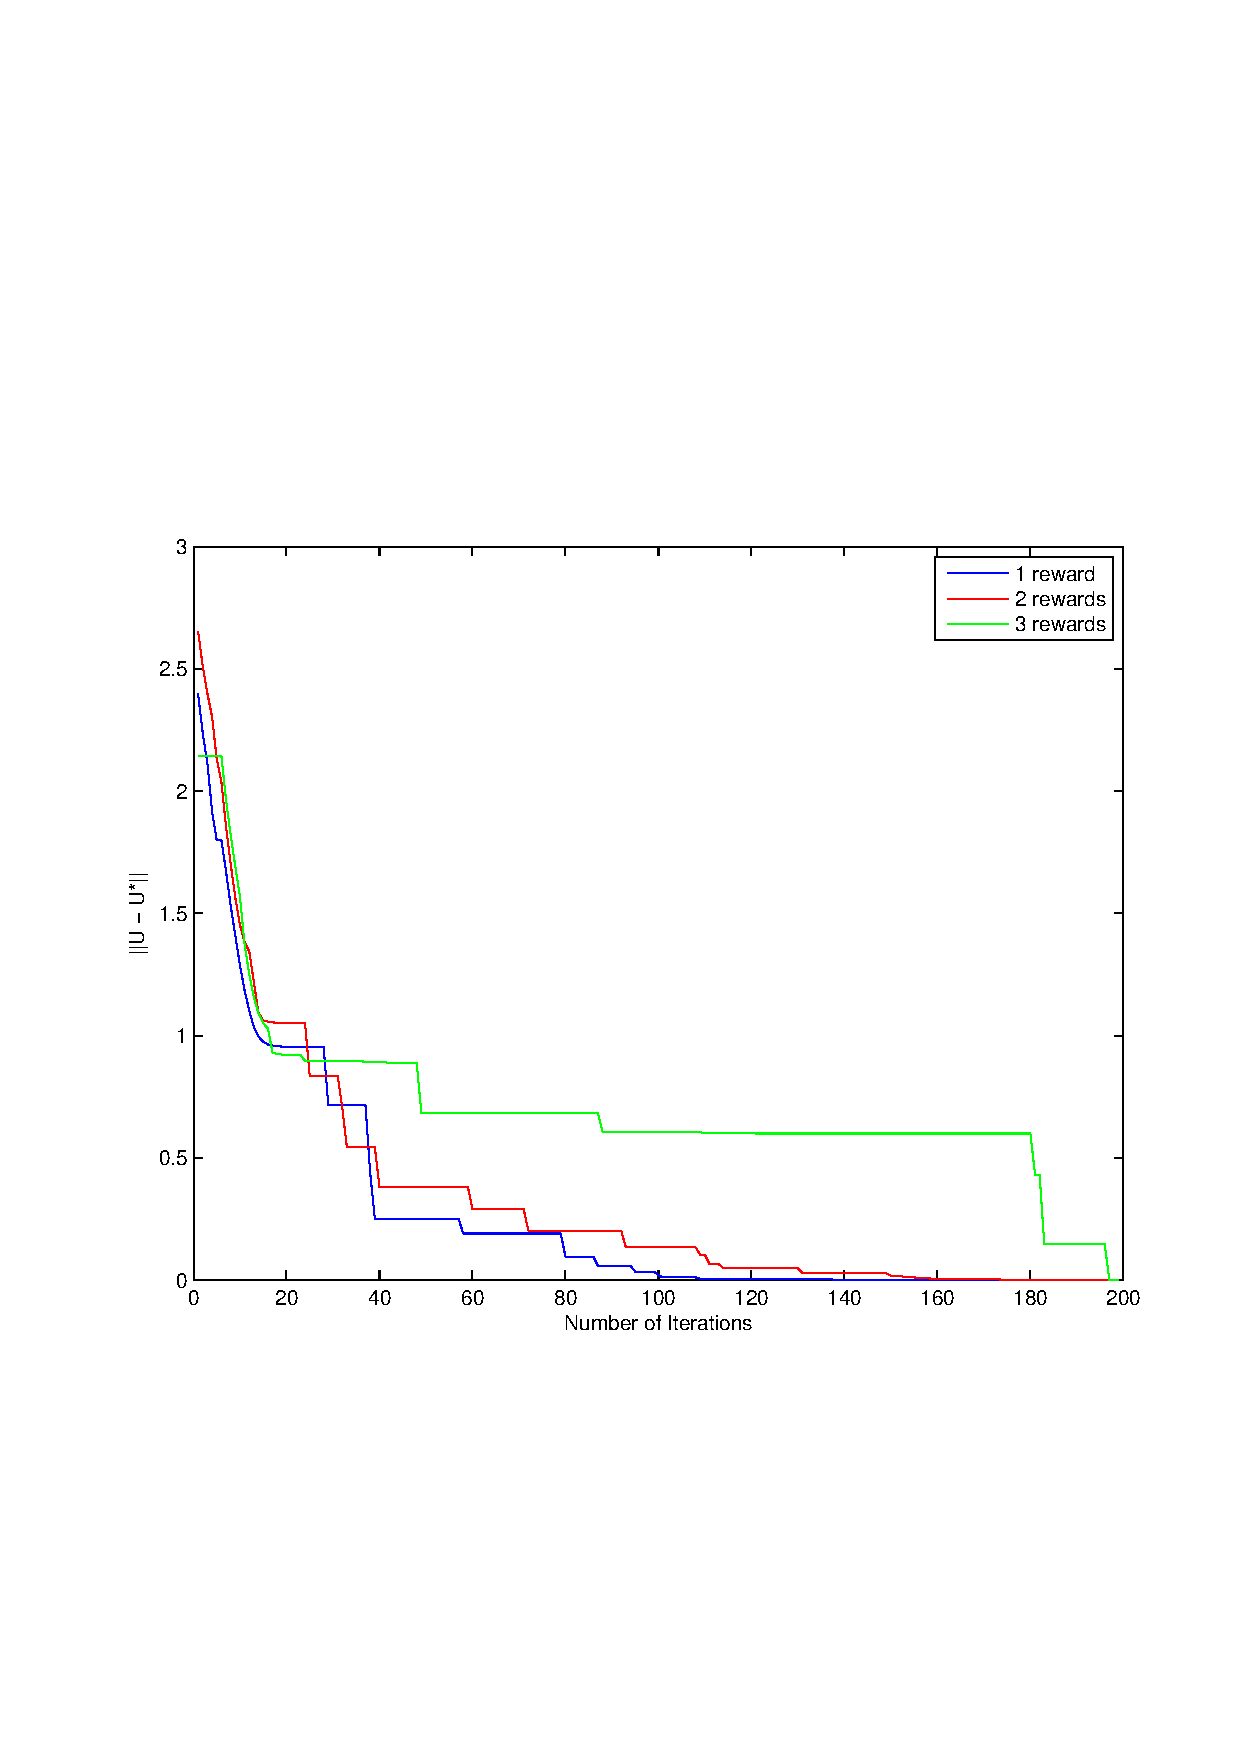
\includegraphics[width=0.7\textwidth]{experiment.pdf}
\caption{Convergence rates of domains of different number of rewards.}
\label{fig:exp}
\end{figure}
\end{frame}

\begin{frame}
\frametitle{E$^3$ Algorithm}
Kearns et al. proposed an algorithm Explicit Explore or Exploit
(E$^3$)\cite{kearns2002near} that uses the mixing time of the domain. The
convergence time of the learning algorithm can be polynomially bounded by the
mixing time of the transition function with high probability.
\end{frame}

\begin{frame}
\frametitle{E$^3$ Algorithm}
\begin{theorem}
Let $U^∗(i)$ denote the value function for the policy with the optimal expected
discounted return in M. Then there exists an algorithm A, taking inputs
$\epsilon,\delta,N$ and $U^∗(i)$,such  that  the  total  number  of  actions  and  computation
time  taken  by  $A$ is  polynomial  in $1/\epsilon,1/\sigma,N$,the mixing time
of the transition function, and the maximum reward. With probability at
least $1-\delta$, $A$  will halt in a state $i$, and output a policy such that
following such policy, $U(i) \geq U^*(i) - \epsilon$.
\end{theorem}
\end{frame}

\begin{frame}
\frametitle{Sketch of E$^3$ Algorithm}
\begin{itemize}
\item Initially, the set $S$ of known states is empty.
\item Any time the current state is not in $S$, the algorithm performs random
walk.
\item Any state that is visited {\em enough times} in the random walk is marked
as {\em known}, and not considered for exploration in the future.
\end{itemize}
\end{frame}

\begin{frame}
\frametitle{Conclusion}
\includegraphics[width=0.7\textwidth]{dopamine.jpg}
\end{frame}

\bibliographystyle{plain}

\bibliography{report}

\end{document}
